The third model considered is proposed by Fu et al. \cite{fu2021fokker}. They
propose a simplified model that expliclty incorporates boundary accummulation. Stochasticity is
only present in the angular variable $\theta$, and there is no shape or hydrodynamic 
forces incorporated, so only a point particle is considered.

The model imposes boundary accumulation by introducing a free-swimming phase (FSP) and two boundary
capture phases, corresponding to interactions with the upper and lower channel walls. In the 
free-swimming phase, the cell swims at a constant speed $U$ while experiencing stochasticity solely
in its angular orientation. Upon contact with either boundary, the cell transitions to a 
boundary-capture phase (BCP), remaining stationary at the boundary until its orientation changes
sufficiently - due to continued rotational Brownian motion - to direct its trajectory away from
the wall. 

The SDEs describing this system are:

\begin{subequations}\label{eq:model_3_sdes}
    \begin{align}
        Y(t + \Delta t) &=
        \begin{cases}
            Y(t) + U \sin(\theta) \Delta t, & \text{if } |Y(t)| \le \frac{H}{2} \text{or } 
            |Y(t)| = \frac{H}{2} \text{and } Y(t) \theta(t) \leq 0 \\
            Y(t), & \text{if } |Y(t)| = \frac{H}{2} \text{and } Y(t) \theta(t) \ge 0
        \end{cases} \\
        \theta(t + \Delta t) &= \theta(t) + \sqrt{2D_{\theta}}dW.
    \end{align}
\end{subequations}

In this model, the vertical coordinate system is centred such that $y=0$ corresponds to the 
midpoint of the chanel, with channel boundaries positioned at $y=\frac{H}{2}$ and 
$y = -\frac{H}{2}$. Additionally, $\theta$ now ranges between $[-\pi, \pi]$. This choice
of coordinates simplifies the conditional statements in equations \eqref{eq:model_3_sdes}.
An illustration of the model is shown in Figure \ref{fig:model_3_setup}. 

\begin{figure}[htbp]
    \centering
    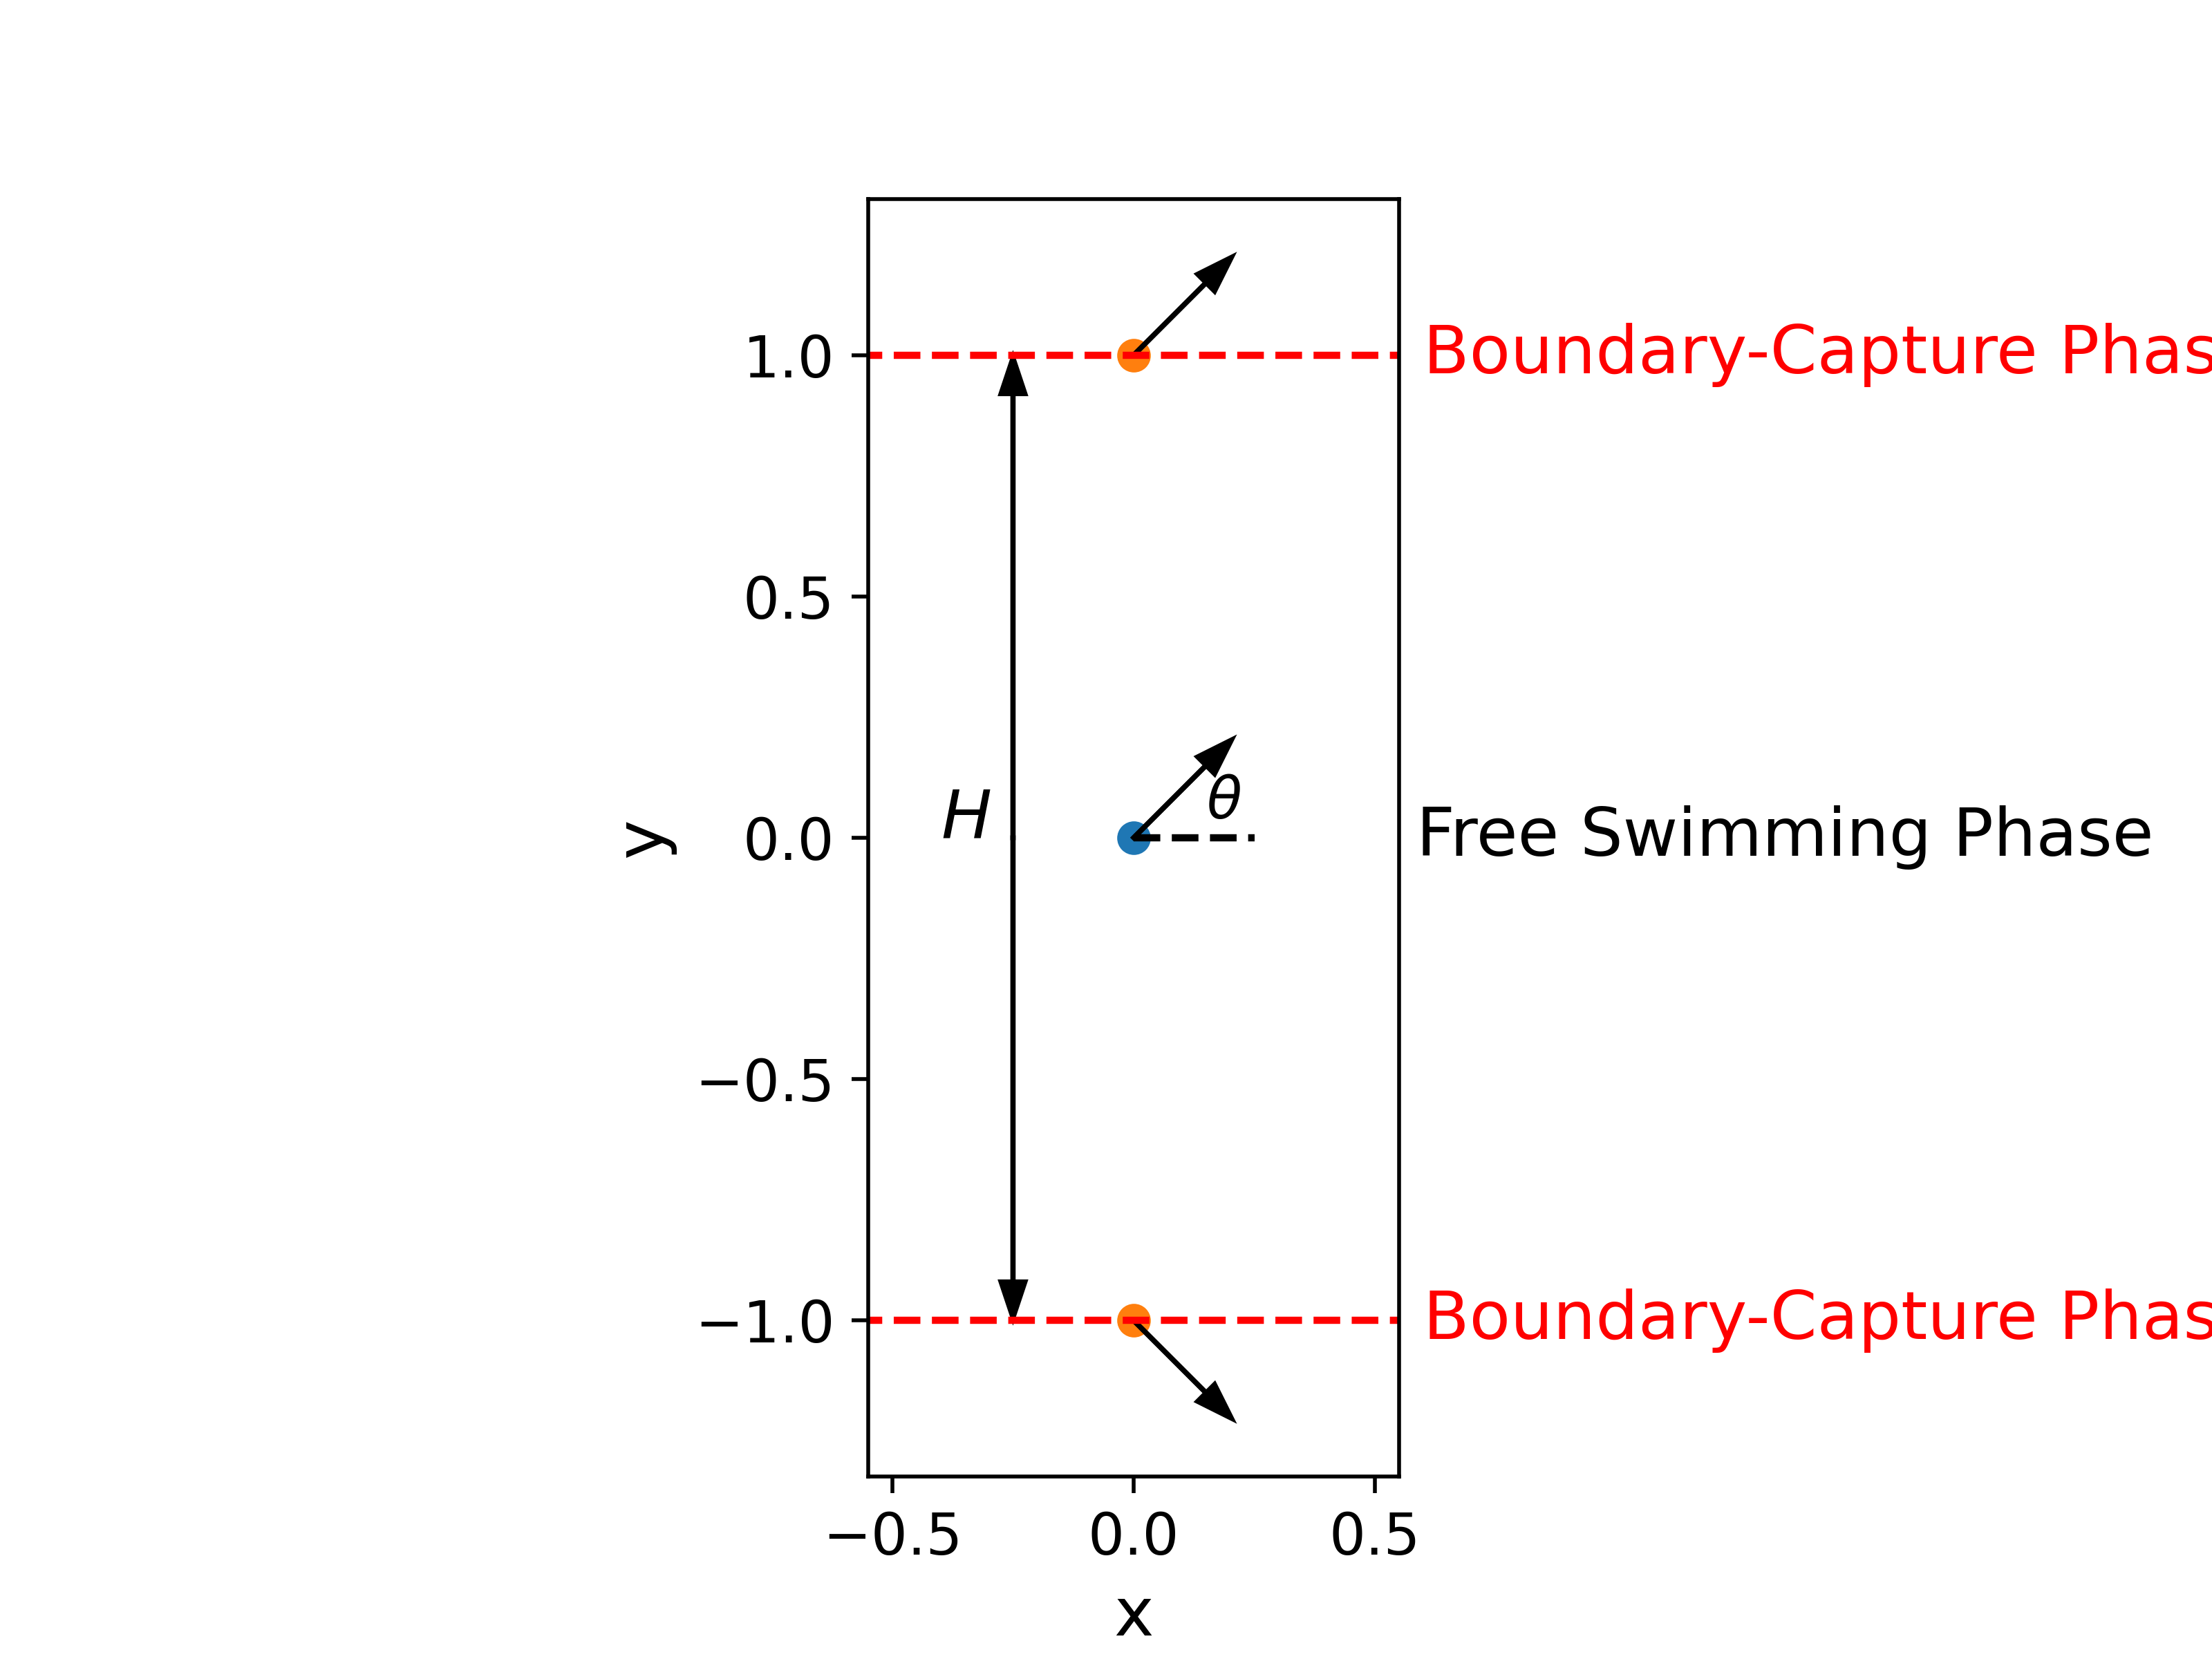
\includegraphics[scale=0.5]{graphics/model_3_setup.png}
    \caption{Schematic illustration of the system configuration for Model 3. Microswimmer is 
    treated as a point particle in a channel of height $H=2$, with boundaries at
    $y=\frac{H}{2}$ and $y=-\frac{H}{2}$. The particle remains trapped at a boundary until 
    its orientation is redirected inward, away from the boundary.}
    \label{fig:model_3_setup}
\end{figure}

The authors propose the following Fokker-Planck system for SDEs \eqref{eq:model_3_sdes}. 
These equations are degenerate, as the particles motion in $y$ is deterministic.

\begin{subequations}\label{eq:model_3_fk}
    \begin{align}
        & \frac{\partial p}{\partial t} + U \sin(\theta) \frac{\partial p}{\partial y} - D_\theta \frac{\partial^2 p}{\partial \theta^2}, \quad (y, \theta) \in \Omega \label{eq:fsp_sde} \\
        & \frac{\partial p_+}{\partial t} - D_\theta \frac{\partial^2 p_+}{\partial \theta^2} = U \sin(\theta)p(t, \frac{H}{2}, \theta), \quad (\frac{H}{2}, \theta), \quad (\frac{H}{2}, \theta) \in \Omega_+ \label{eq:bcp_sde_up}\\
        & \frac{\partial p_-}{\partial t} - D_\theta \frac{\partial^2 p_+}{\partial \theta^2} = -U \sin(\theta)p(t, -\frac{H}{2}, \theta), \quad (\frac{H}{2}, \theta), \quad (-\frac{H}{2}, \theta) \in \Omega_+ \label{eq:bcp_sde_down}
    \end{align}
\end{subequations}

where $p(t, y, \theta)$ is the PDF of the cells in the FSP at time $t$, position $y$ with orientation $\theta$, while
 $p_\pm$ are the PDFs 
of boundary contacting cells at time $t$, position $\pm \frac{H}{2}$ with non-inward facing orientation. $\Omega$ 
denotes the domain occupied by cells in FSP, while $\Omega_\pm$is the domains of the 
upper and lower BCPs, respectively. 

The associated boundary conditions for \eqref{eq:model_3_fk} are as follows. First we consider the boundary
conditions associated with cells in the FSP \eqref{eq:fsp_sde}. As 
cells with direction $\theta = \pi$ and $\theta = -\pi$ are the same, we have periodic boundary 
conditions in $\theta$:

\begin{equation}
    p(t, y, -\pi) = p(t, y, \pi), \qquad \frac{\partial p}{\partial \theta}(t, y, -\pi) = \frac{\partial p}{\partial \theta},  \qquad -\frac{H}{2} < y < \frac{H}{2}
\end{equation}

Further, as it is impossible for cells in the BCP with outward-facing orientation to enter 
the FSP, we impose Dirichlet boundary conditions at the channel walls:

\begin{equation}
    p(t, L, \theta) = 0, \quad \theta \in (-\pi, 0), \qquad p(t, -L, \theta) = 0, \quad \theta \in (0, \pi).
\end{equation}

For cells in the BCP described by \eqref{eq:bcp_sde_up}, \eqref{eq:bcp_sde_down}, the cells exit this phase once
their orientation points inward, resulting in Dirichlet boundaries in BCP at
$\theta = 0$, $\theta = \pm \pi$:

\begin{equation}
    p_+(t, 0) = p_+(t, \pi) = 0, \qquad p_-(t, 0) = p_-(t, -\pi) = 0.
\end{equation}

Transitions between phases are characterised by source and sink terms, which represent probability 
fluxes between the BCP and FSP. These fluxes are described by the following conditions:

\begin{subequations}
    \begin{align}
        \frac{\partial p}{\partial \theta}(t, y, \theta)\Bigr|_{\theta=\pi_-}^{\theta = \pi_+} = 
        \frac{\partial p_+}{\partial \theta}(t, \pi_-)\delta_{y = \frac{H}{2}} 
        - \frac{\partial p_-}{\partial \theta}(t, \pi_+)\delta_{y=-\frac{H}{2}}\\
        \frac{\partial p}{\partial \theta}(t, y, \theta)\Bigr|_{\theta=0_-}^{\theta = 0_+} = 
        -\frac{\partial p_+}{\partial \theta}(t, 0_+)\delta_{y = \frac{H}{2}} 
        + \frac{\partial p_-}{\partial \theta}(t, 0_-)\delta_{y=-\frac{H}{2}}
    \end{align}
\end{subequations}

The convergece of this system is analysed by Fu et al. \cite{fu2021fokker}, and solved 
via a finite difference scheme on a stencil depicted in Figure \ref{fig:model_3_stencil}.

\begin{figure}[htbp]
    \centering
    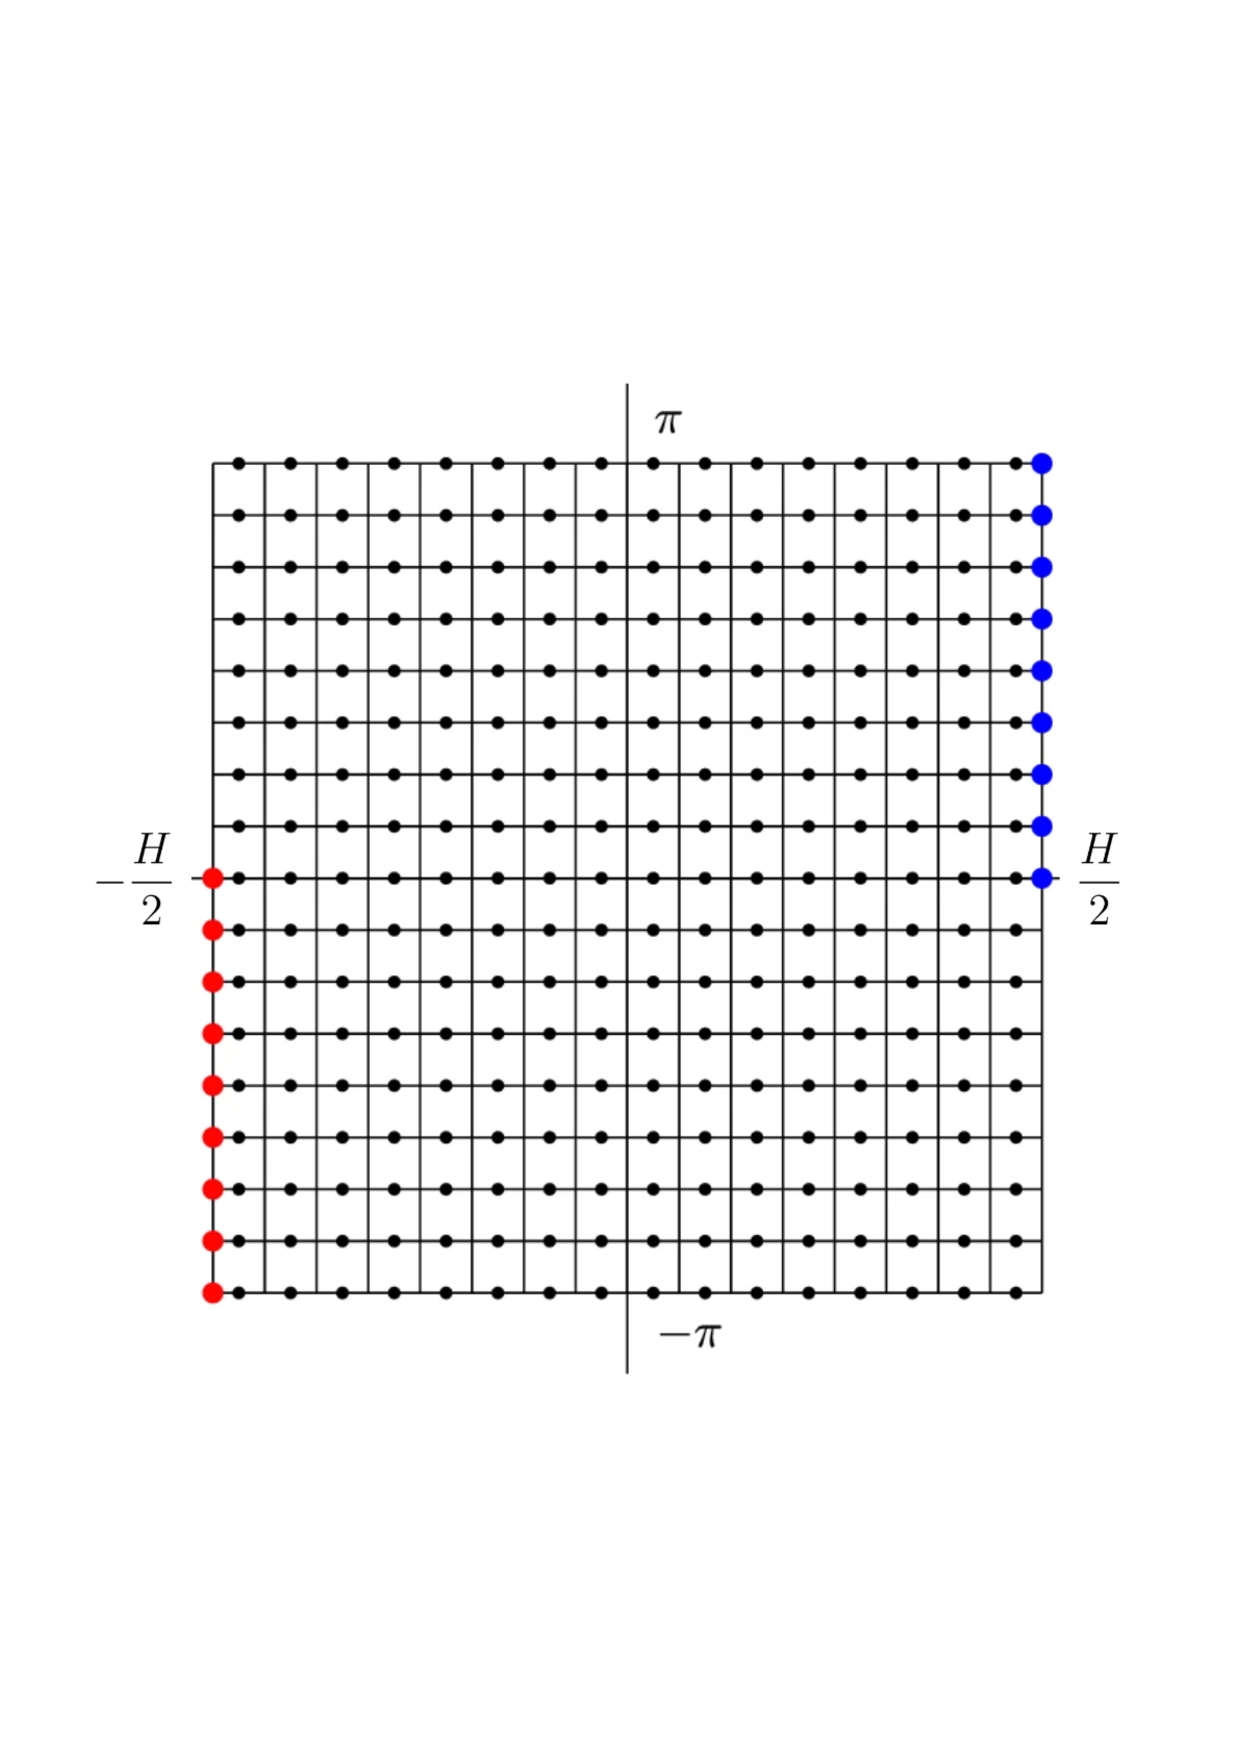
\includegraphics[scale=0.4]{graphics/model_3_stencil.pdf}
    \caption{Stencil of finite difference scheme implemented to obtain stationary distribution for \eqref{eq:model_3_fk}.
    Red dots correspond to nodes in the lower BCP, blue dots correspond to nodes in the upper BCP.}
    \label{fig:model_3_stencil}
\end{figure}


We employed both the finite-difference scheme and Monte Carlo simulations to obtain the stationary distribution 
corresopnding to equations \eqref{eq:model_3_fk}. The resulting PDF and marginal distribution is presented in 
\ref{fig:model_3_results}.

\begin{figure}[htbp]
    \centering
    \begin{subfigure}[b]{0.45\textwidth}
        \centering
        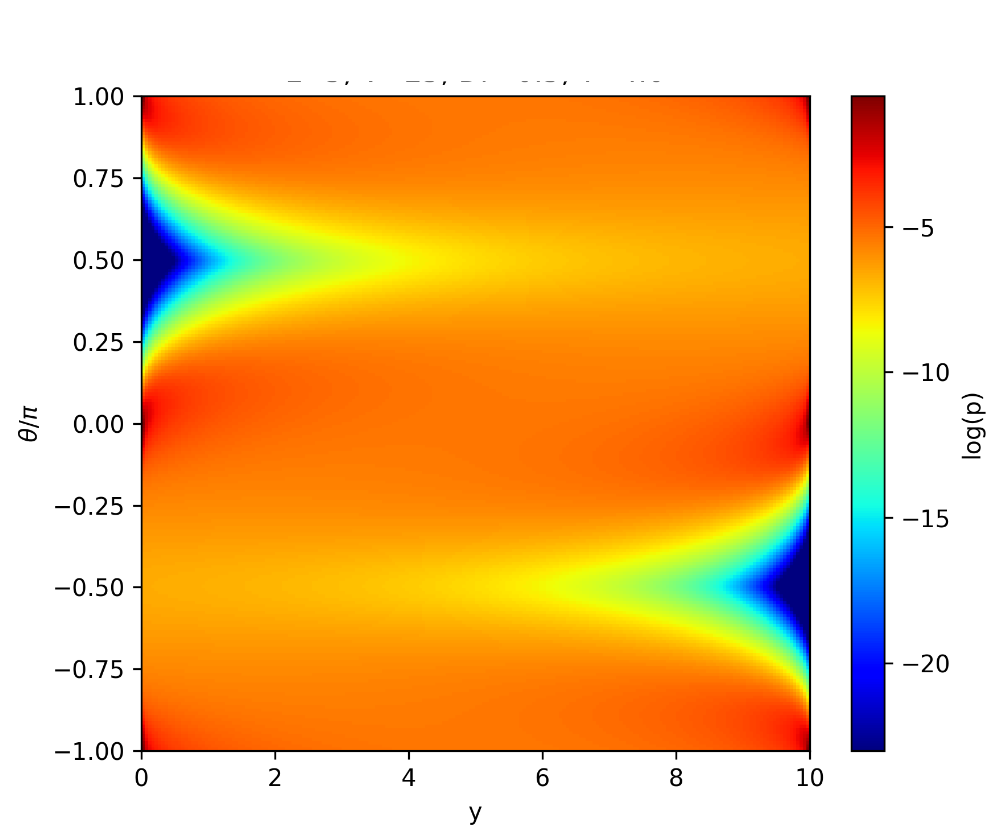
\includegraphics[scale=0.2]{graphics/model_3_pdf.png}
        \caption{Heatmap of stationary distribution obtained from \eqref{eq:model_3_fk}. 
        Parameters are: $H=10$, $U=25$, $D_\theta$=0.5.}
        \label{fig:model_3_pdf}
    \end{subfigure}
    \hfill
    \begin{subfigure}[b]{0.45\textwidth}
        \centering
        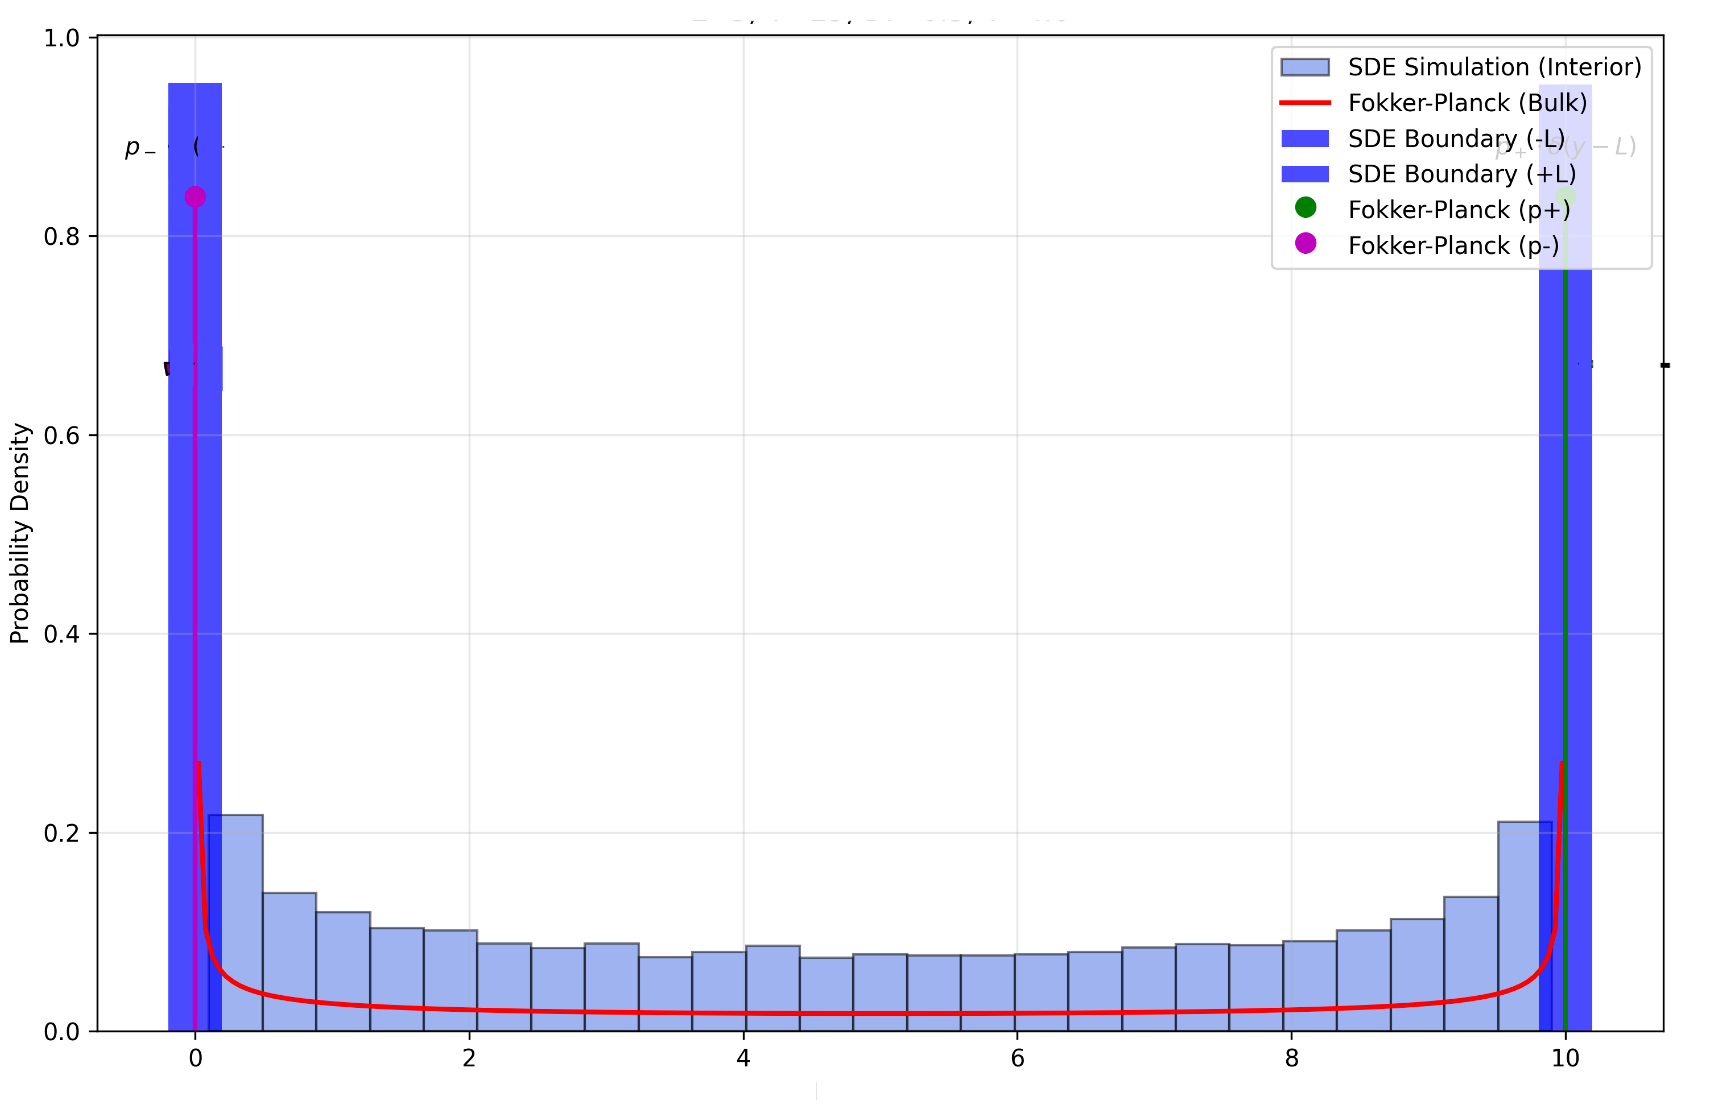
\includegraphics[width=\textwidth]{graphics/model_3_hist.png}
        \caption{Marginal distribution along the channel obtained by Monte Carlo (histogram) and 
        finite-difference scheme (solid lines).}
        \label{fig:model_3_hist}
    \end{subfigure}
    \caption{Stationary and marginal distributions for the system described by equations~\eqref{eq:model_3_fk}.}
    \label{fig:model_3_results}
\end{figure}

Figure \ref{fig:model_3_hist} demonstrates the characteristic boundary accumulation, which is expected 
given that boundary accumulation isexplicitly built into this model. Additionally, Figure \ref{fig:model_3_pdf} 
exhibits regions of extremely low probability density in the upper-left and lower-right corners. These correspond 
to regions where the cell's motion is directed opposite to its vertical orientation, making such configurations 
highly unlikely. The probability is $0$ in these regions directly against the boundary, as it is impossible for 
the cell to exit the BCP while its orrientation is against the opposite channel.



